\chapter{Конструкторский раздел}
\label{cha:design}

В данном разделе рассматривается проектирование структуры программного обеспечения и требования к нему.

\section{Функциональная модель предлагаемого метода}

На рис. \ref{fig:idef0} представлена функциональная схема предлагаемого метода 
определения признаков авторского стиля в нотации IDEF0, нулевой уровень.

\begin{figure}[H]
    \centering
    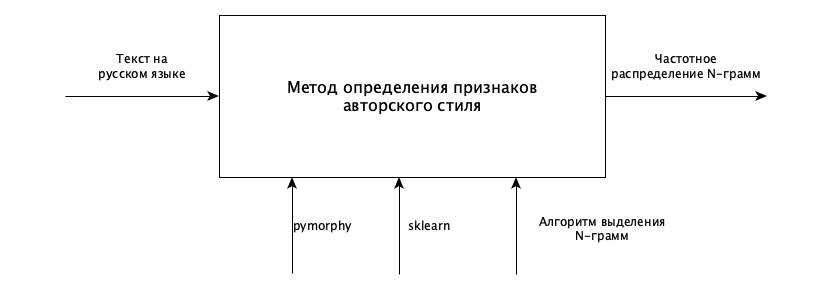
\includegraphics[scale=0.5]{img/idef0.png}
    \caption{Функциональная схема метода определения признаков авторского стиля}
    \label{fig:idef0}
\end{figure}

\section{Требования к программному обеспечению}

Необходимо разработать программное обеспечение, которое получает на вход текст на русском языке, и с помощью метода выделения N-грамм определяет признаки текста: морфологические параметры N-грамм, мера TF\_IDF. На выходе получаем частотное распределение N-грамм с определенными частями речи.

\section{Выводы}

В данном разделе был рассмотрен процесс проектирования структуры программного обеспечения и требования, выдвигаемые  к программному обеспечению.
